\setchapterstyle{kao}
\setchapterpreamble[u]{\margintoc}
\chapter{Neutrinos in High Energy Universe}
\labch{nu_theory_sources}
\begin{figure}[h]
    \caption{Measured and predicted neutrino fluxes of neutrinos from various natural sources. Solar neutrinos are neutrinos, while geo-neutrinos and nuclear reactors (terrestrial) are antineutrinos. Other sources produce roughly equal numbers of neutrinos and antineutrinos. Neutrinos from the Big Bang, diffuse supernova neutrinos, and high-energy cosmogenic neutrinos remain undetected. Figure from \cite{KATZ2012651}}
    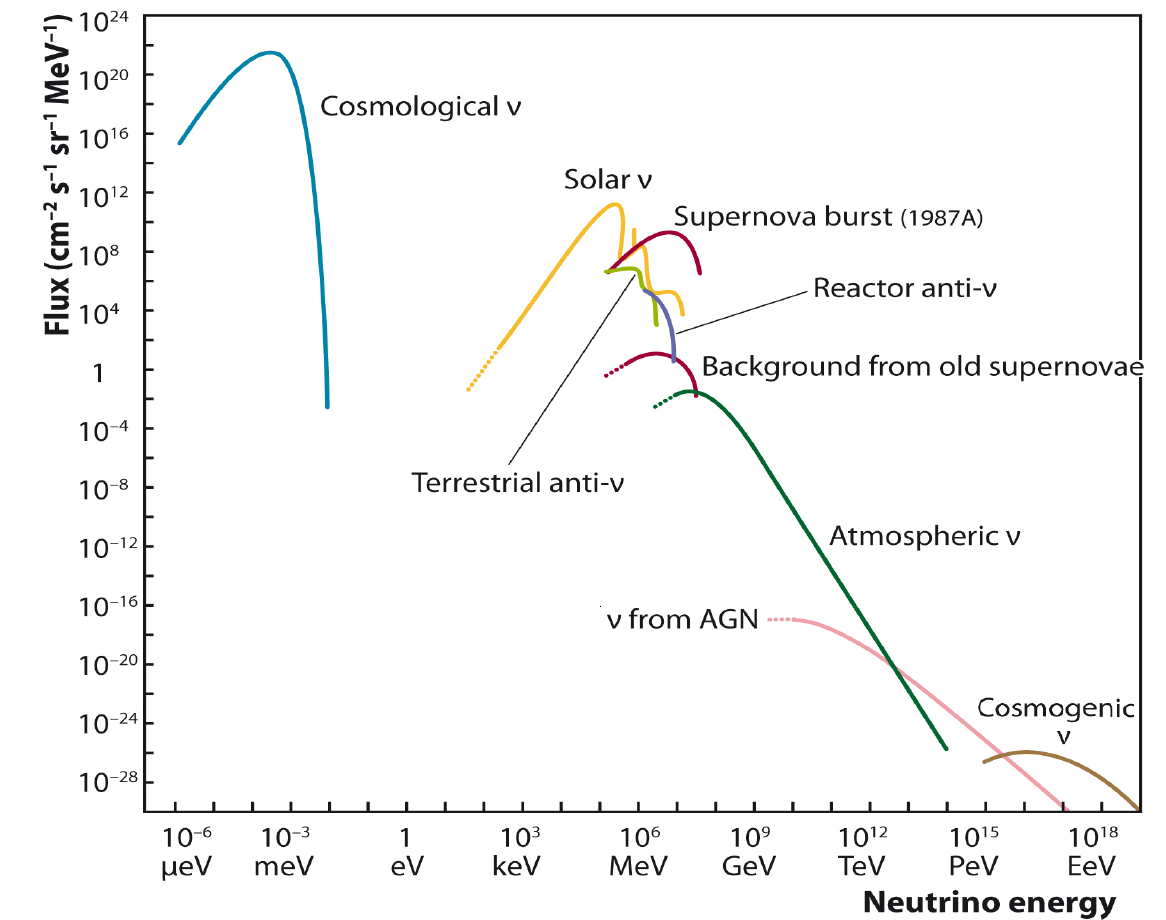
\includegraphics{./figures/nu_phenomenology/all-nu-spectrum-mod.png}
    \labfig{nu_spectrum}
\end{figure}
Neutrinos are produced by various sources across a very large energy range (see \reffig{nu_spectrum}), including particle accelerators, nuclear reactors, and several natural processes. The largest flux of neutrinos comes from nuclear fusion in the Sun \sidecite{Bahcall} and naturally occurring $\beta$-decay on Earth (the so-called \emph{GeoNeutrinos} or \emph{terrestrial neutrinos}) \sidecite{Krauss}. Historically, a similar flux was briefly observed during the supernova SN1987a in the Large Magellanic Cloud, though it only lasted a few seconds \sidecite{SN1987A_superK,SN1987A_Baksan,SN1987A_IMB}. A more constant, but significantly lower, flux is thought to arise from numerous supernovae throughout the universe \sidecite{Vissani}. High-energy neutrinos, above 1 TeV, originate from either atmospheric or astrophysical sources and are of particular interest for the work presented in this thesis. 

As high-energy neutrinos (above tens of TeV) are expected to be produced alongside cosmic rays at high-energy acceleration sites, this chapter will first introduce cosmic rays. It will then cover the production of neutrinos and muons from cosmic ray interactions with Earth's atmosphere, followed by a discussion on neutrinos generated at cosmic ray acceleration sites.

\section{Cosmic Rays}
\label{sec:cosmic_rays}
Cosmic rays were first discovered by Victor Hess during his famous balloon flight in 1912, where he measured a significant increase in ionization rates as he ascended in altitude \sidecite{HESS_Balloon}. This finding provided the first direct evidence for the existence of highly energetic particles arriving from outer space. Over a century later, cosmic ray research has evolved, and today various experiments routinely measure their physical properties. Cosmic rays are now understood to consist primarily of ionized atomic nuclei, with less than 1\% of their composition being electrons, which are often disregarded due to their negligible contribution. Approximately 90\% of cosmic rays are protons, 9\% are helium nuclei ($\alpha$-particles), and the remaining fraction consists of heavier nuclei such as carbon, oxygen, and iron \sidecite{PDG2022}.

Cosmic radiation that reaches the Earth's atmosphere contains all stable charged particles and atomic nuclei with lifetimes of $10^6$ years or more. These particles are divided into \emph{primary} and \emph{secondary} cosmic rays. Primary cosmic rays are particles that are directly accelerated by astrophysical sources. These include protons, helium nuclei, and heavier elements formed in stars. On the other hand, secondary cosmic rays are produced when primary cosmic rays interact with interstellar matter. For example, when primary cosmic rays hit gas particles in space, they can create lighter elements like lithium, beryllium, and boron, which are not typically formed in stars. These secondary particles help scientists understand the interactions cosmic rays experience as they travel through the galaxy \sidecite{PDG2022}.

\begin{figure}[h]
    \caption{The all-particle spectrum as a function of E (energy-per-nucleus) from air shower measurements. The various features of the spectrum discussed in the text are marked with \emph{Knee, 2nd Knee and Ankle}. Data points are referenced in \cite{PDG2022}}
    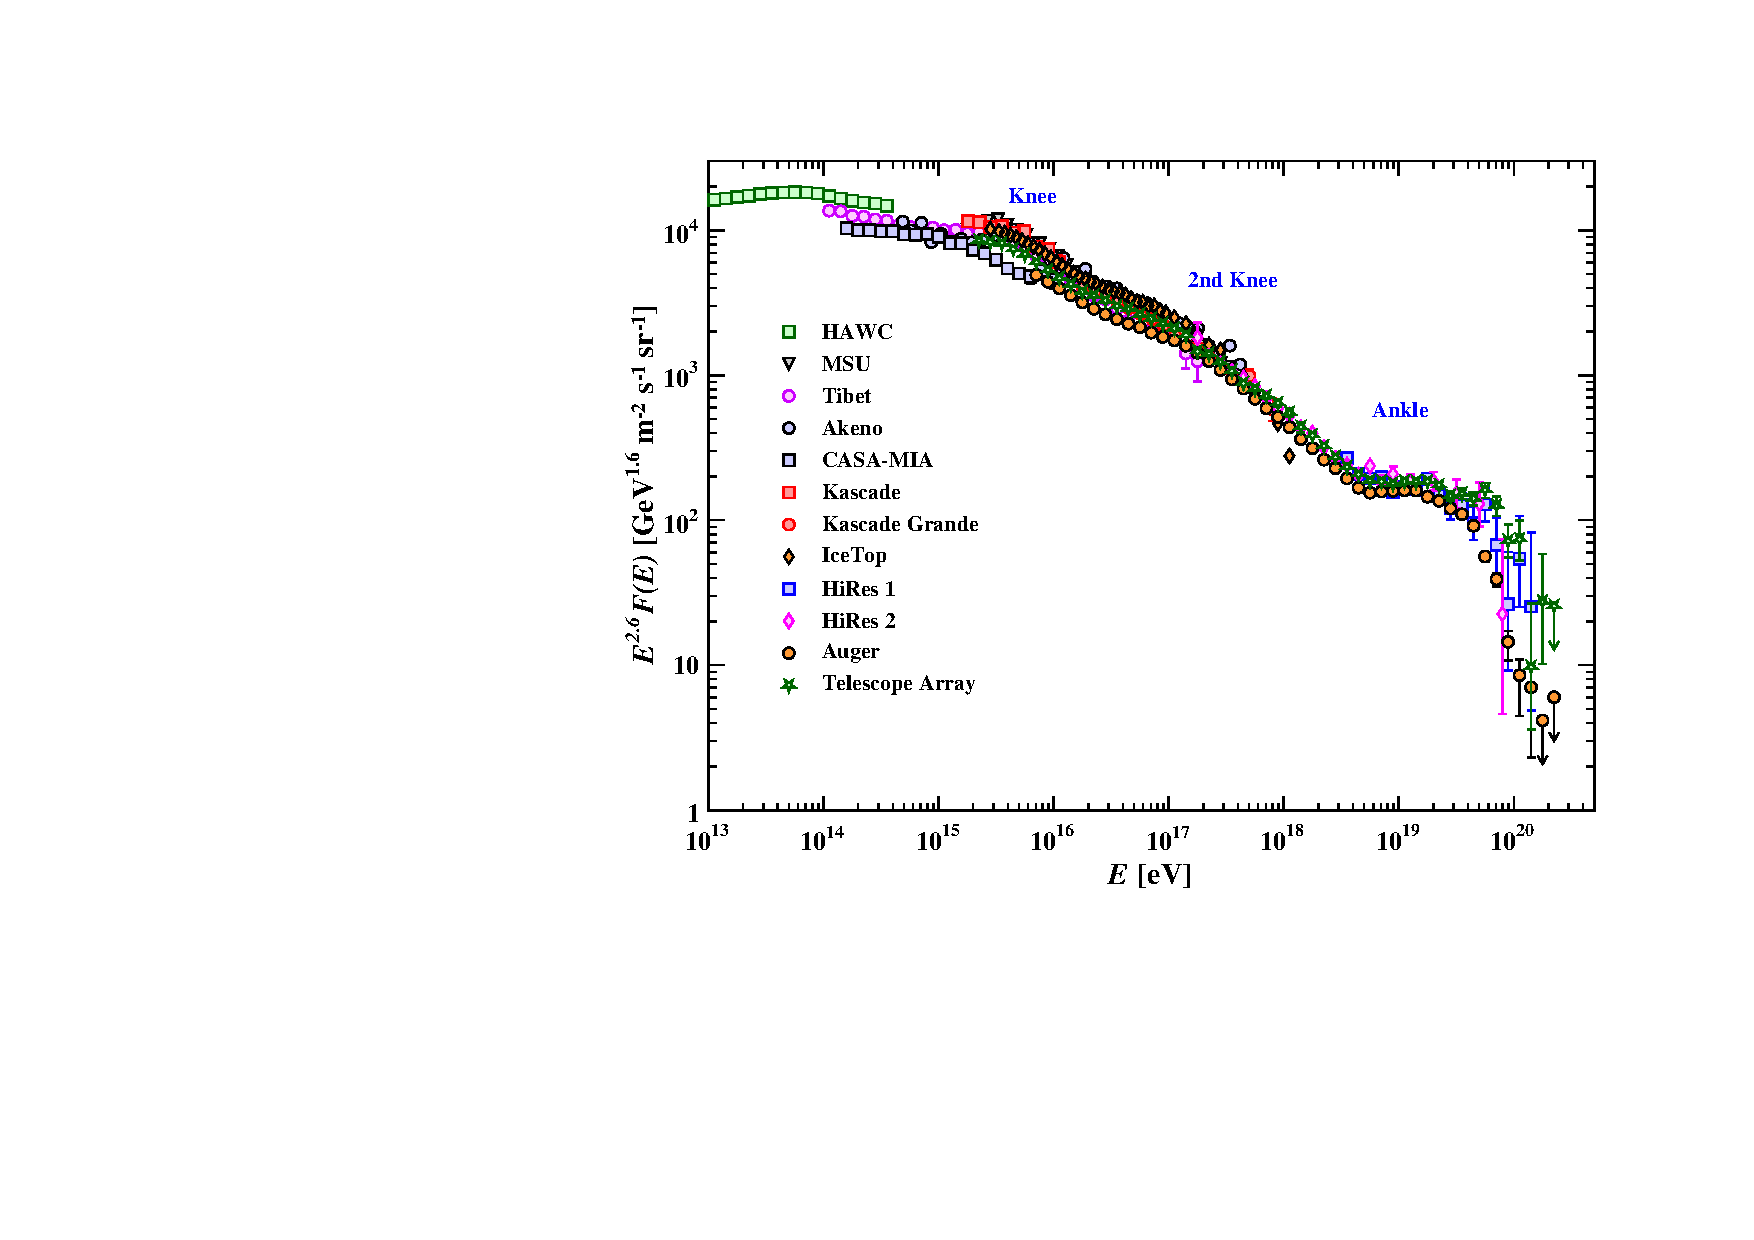
\includegraphics{./figures/nu_he/cr_fig8_AllParticle_21.pdf}
    \labfig{cosmicray_spectrum}
\end{figure}

The energy spectrum of cosmic rays as shown in \reffig{cosmicray_spectrum} is one of their most fascinating characteristics.. The spectrum follows a power-law distribution, expressed as:

\begin{equation}\label{eq:flux}
\frac{dN}{dE} \propto E^{-\gamma}
\end{equation}


where \( E \) is the energy and \( \gamma \) is the spectral index. This form of the spectrum indicates that cosmic rays are accelerated by non-thermal processes, such as shock waves or magnetic reconnection. The spectral index \( \gamma \) is not constant across all energies but changes at specific points in the spectrum (as indicated in \reffig{cosmicray_spectrum}), indicating transitions between different source classes or acceleration mechanisms. Over a vast energy range (from $\sim10^9 \, \mathrm{eV} \, \mathrm{to} \, \sim 10^{15} $), the differential flux given in Equation~\ref{eq:flux} follows a power law with index $\gamma\approx2.7$. The flux in this range, is large enough to be measured be directly detected from spacecraft and balloons before they interact in the atmosphere. 

\marginnote{\begin{kaobox}
    The various features \cite{PDG2022} that can be seen in the \reffig{cosmicray_spectrum} using Equation~\ref{eq:flux} are as follows:
    \begin{equation*}
        \frac{dN}{dE} \sim
            \begin{cases}
            E^{-2.7} & \text{(up to knee)}\\ 
            E^{-3.1} & \text{(knee) }  \\
            E^{-3.3} & \text{(second knee)} , \\
            E^{-2.5} & \text{(ankle)}
            \end{cases}
    \end{equation*}
\end{kaobox}} 

At higher energies, where the cosmic ray flux is too low to be measured directly, they can only be observed indirectly through the cascade of secondary particles they produce in the atmosphere. The energy and type of the primary cosmic ray must then be estimated based on the characteristics of this particle shower. The first significant feature in the cosmic ray energy spectrum is known as \textbf{the knee}, which occurs at an energy of about 3 PeV. At this point, the spectrum softens, with the spectral index \( \gamma \) increasing from around 2.7 to about 3.1. A milder, \textbf{second knee} occurs at around \( 10^{17} \, \text{eV} \) (100 PeV), where the spectrum softens further to $\gamma\sim3.3$.  The Cosmic rays above \( \sim10^{18} \, \text{eV} \) are called \emph{Ultra High Energy Cosmic Rays (UHECRs)}. At these ultra higher energies, the spectrum undergoes a hardening at around \( 10^{18} \, \text{eV} \), where the index returns to a value closer to 2.5. This feature of the spectrum is known as \textbf{ankle} \sidecite{H_RANDEL_2007}. At the highest energies, specifically beyond \(10^{18}\) eV, a decline in cosmic ray flux is expected. This decrease can be explained by \textbf{the Greisen-Zatsepin-Kuzmin (GZK)} mechanism, which involves the production of pions through photohadronic interactions between high-energy protons (E$\sim$50 EeV ($50\times10^{18}$ eV)) and photons from the cosmic microwave background (CMB) \sidecite{GZK1,GZK2}. For this GZK effect to fully account for the observed spectral cutoff, a proton-only composition is necessary. However, data from the Pierre Auger Observatory (PAO) and the Telescope Array (TA) suggest otherwise, indicating a more mixed composition \sidecite{Ankle_AugerPaper,auger_ta_joint}. Another possible explanation for the observed flux suppression is the finite maximum energy that cosmic ray sources can accelerate particles to \sidecite{Das_2021}.

These transitions in the spectrum are believed to be associated with changes in the source population. The initial segment of the cosmic ray energy spectrum, extending up to the knee can largely be explained by the process of particle acceleration occurring within Galactic sources, predominantly supernova remnants \sidecite{modelling}. Supernova remnants serve as dynamic environments where powerful shock waves are generated following the explosive death of massive stars. These shock waves facilitate the acceleration of particles, including protons, to high energies through mechanisms such as Fermi acceleration (see below) \sidecite{Perkins}. The steepening of the spectrum at the knee suggests that accelerators may have reached their maximum capacity for proton acceleration  \sidecite{H_randel_2003}. This limit depends largely on the strength of magnetic fields in the acceleration region, which are crucial for confining charged particles and facilitating energy gain. Additionally, cosmic ray leakage from the Galaxy can reduce high-energy cosmic rays through interactions with interstellar medium particles, contributing to the observed changes in the energy spectrum \sidecite{somthingCR}. 

The second knee in the cosmic ray spectrum can also be understood using similar principles. This feature may arise from the behavior of heavier elements, which experience different acceleration dynamics compared to protons \sidecite{H_randel_2003}. These heavy nuclei may encounter limitations in their acceleration processes, preventing them from reaching energies comparable to lighter particles. Moreover, just like protons, these heavier elements may also face barriers that inhibit their escape from the Galactic environment. Consequently, the second knee could signify a threshold beyond which heavier cosmic rays cannot be further accelerated or are unable to exit the Galaxy, leading to a corresponding steepening in the spectrum. Overall, these observations underscore the complex interplay between acceleration mechanisms, magnetic field strengths, and particle interactions that shape the cosmic ray energy spectrum. Regarding the ankle region, several proposed models that seek to explain this phenomenon suggest a transition in the primary component from galactic sources to extragalactic ones \sidecite{ankle1,ankle2,ankle3}. 

Anisotropies in the arrival directions of cosmic rays (CRs) offer crucial insights into their origins. Identifying these sources becomes theoretically possible if the properties of cosmic ray charges, as well as galactic and extragalactic magnetic fields, are sufficiently well understood. Ultra-high-energy cosmic rays (UHECRs) are notably affected by the Greisen-Zatsepin-Kuzmin (GZK) effect, which describes the energy losses experienced by protons and heavier nuclei due to their interactions with the cosmic microwave background. The Pierre Auger Observatory has identified a large-scale dipolar anisotropy in cosmic rays with energies above 8 EeV, with a significance of $6.9\sigma$. The amplitude of this dipole is $d = 0.073^{+0.010}_{-0.008}$, and its direction is approximately $115^\circ$ away from the Galactic Center, supporting the extragalactic origin of UHECRs beyond this energy threshold \sidecite{anisotropy_PAO}. These findings align with results obtained by combining the data from both the Pierre Auger Observatory and the Telescope Array (TA) \sidecite{anisotropy_TA}.

\subsection{Acceleration Mechanism}
\label{sec:accln}
Even during the most powerful solar flares, the Sun is limited to accelerating particles to around 1 GeV \sidecite{solar_flare}. This limitation leads to the question of how cosmic rays can be accelerated to much higher energies, ranging from tens of GeV up to 100 EeV, and what astrophysical sources and mechanisms are responsible for such acceleration. One leading theory, initially proposed by Enrico Fermi, is that cosmic ray particles gain energy through random scattering across moving shock fronts, a process known as first-order Fermi acceleration \sidecite{fermi_accln}. In this process, the relative energy gain $\Delta E$ for a particle with energy $E$ during each scattering event is proportional to the shock velocity $u$, expressed by the equation:

\begin{equation}
    \frac{\Delta E}{E} \sim \frac{u}{c},
\end{equation}

where $c$ is the speed of light \sidecite{Gaisser_Engel_Resconi_2016}. \sidenote{For instance, supernova remnants, where the shock front velocity $u/c \gtrsim 10^{-2}$, create a highly efficient environment for particle acceleration.} A charged particle, starting in the unshocked region, moves into the shocked medium and experiences elastic scattering from magnetic irregularities. With every crossing of the shock front, the particle gains more energy. After $n$ cycles, the particle's energy is given by $E_n = E_0(1 + \alpha)^n$, where $E_0$ is its initial energy and $\alpha$ represents the fractional energy increase per cycle, approximately $\alpha \approx 4v/3c$ \sidecite{Gaisser_Engel_Resconi_2016}. However, particles cannot remain in the shock zone indefinitely, as they may either just loose the energy or \emph{escape} the region. The latter is determined by their escape probability, $p_{\text{esc}} = 4(u - v)/c$, which increases as the shock slows down relative to the surrounding medium.

The resulting energy spectrum of the accelerated particles typically follows a power law, with the differential energy distribution given by $dN/dE \propto E^{-\gamma}$, where $\gamma \approx 1 + \frac{p_{\text{esc}}}{\alpha}$ \sidecite{Perkins}. In non-relativistic shocks moving faster than the speed of sound in the medium, this leads to a spectral index of approximately $\gamma \approx 2.1$, meaning most particles have lower energies, while a smaller number reach higher energies. The steeper cosmic ray spectrum, approximately $\sim E^{-2.7}$, can be explained by energy-dependent diffusion in galactic magnetic fields \sidecite{Batista_2014,Snodin:2015fza}.

Although first-order Fermi acceleration is a strong model for non-relativistic shocks, other mechanisms have been proposed to account for even higher-energy particles. These include relativistic shock fronts \sidecite{1987ApJ,1988MNRAS}, where shocks travel close to the speed of light, as well as processes like magnetic reconnection \sidecite{RevModPhys.82.603}, where energy is released when magnetic fields reconfigure, and plasma wakefield acceleration \sidecite{Chang:2007um}, where particles are accelerated by intense electric fields in plasmas. Such processes are crucial in extreme astrophysical environments like active galactic nuclei (AGN) and gamma-ray bursts (GRBs), where cosmic rays are believed to be accelerated to ultra-high energies.

\subsection{Sources}
\label{sec:cosmic_sources}
The notion of Fermi acceleration, as explained in Section~\ref{sec:accln} fundamentally relies on the confinement of cosmic rays, which allows them to engage in repeated interactions with a shock front or other magnetized structures. If we assume that this confinement is provided by a magnetic field of strength \(B\), it follows that the size of the confinement region, denoted as \(r\), must be greater than the gyro-radius of the cosmic ray. This relationship is described by the following inequality:

\begin{equation}
    r > \frac{E}{ZBc}
\end{equation}

Here, \(E\) represents the energy and \(Z\) is the charge of the cosmic ray, which we typically consider to be ultra-relativistic. Alternatively, this condition can be reformulated as a constraint on the rigidity \(R\), defined as the ratio of the particle's momentum to its charge:

\begin{equation}
    R = \frac{E}{Z} < Bcr.
\end{equation}

\begin{figure}[h]
    \caption{Hillas diagram illustrating different candidate source classes of cos- mic rays. Figure from \cite{hillas_plot}}
    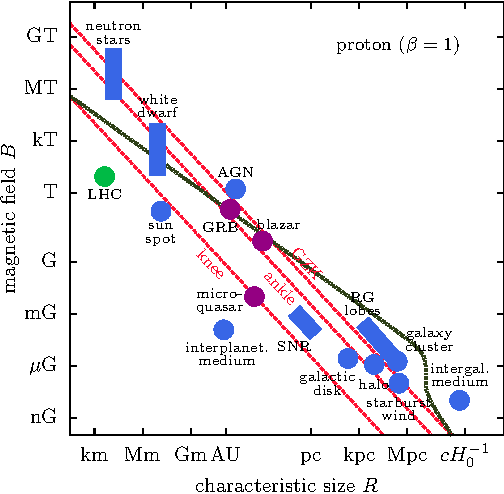
\includegraphics{./figures/nu_he/Hillas_simple.pdf}
    \labfig{hillas}
\end{figure}

This limitation is referred to as \textbf{the Hillas criterion} \sidecite{hillas}. By employing estimates for the sizes and magnetic field strengths of various astronomical objects, one can identify potential sites for acceleration that align with specific cosmic-ray rigidities. The Hillas diagram as shown in \reffig{hillas}, effectively illustrates the magnetic field strength and sizes of different classes of objects.

Following the aforementioned concept, Hillas proposed a simple model that captures the characteristics observed in the energy spectrum and composition of cosmic rays. In this framework, the diagonal lines in \reffig{hillas} signify thresholds below which a source cannot confine a particle with energy \(E\) and charge \(z\). Considering that the Milky Way has a thickness of no more than 1 kpc \sidecite{Rix:2013bi} and its magnetic field strength is approximately a few $\mu G$ \sidecite{Haverkorn:2014jka}, the Hillas diagram suggests that UHECRs must originate from extragalactic sources. Conversely, galactic supernova remnants (SNRs) emerge as strong candidates for the source of low-energy cosmic rays. While the exact rate of galactic supernova occurrences remains somewhat uncertain, a conversion of just a few percent of the shock wave's energy into particle acceleration would adequately explain the observed cosmic ray flux  below the knee of the cosmic ray spectrum \sidecite{Perkins}.

The origins of cosmic rays in the intermediate energy range (between knee and second knee) are still not fully understood \sidecite{Halzen:2010yj}. Their acceleration is thought to take place within vast magnetic fields generated by substantial bulk flows of relativistic charged particles, which are driven by immense gravitational forces present in the vicinity of neutron stars or black holes. Some plausible candidates for these highest-energy cosmic rays include \textbf{Active Galactic Nuclei (AGN)} \sidecite{Protheroe:1992qs} and \textbf{Gamma-Ray Bursts (GRB)} \sidecite{Wang:2007xj}. 
\begin{marginfigure}
    \caption{Schematic of the AGN Unification Model, illustrating AGN structures and how observed properties vary by viewing angle.Figure from \cite{AGN_picture}}
    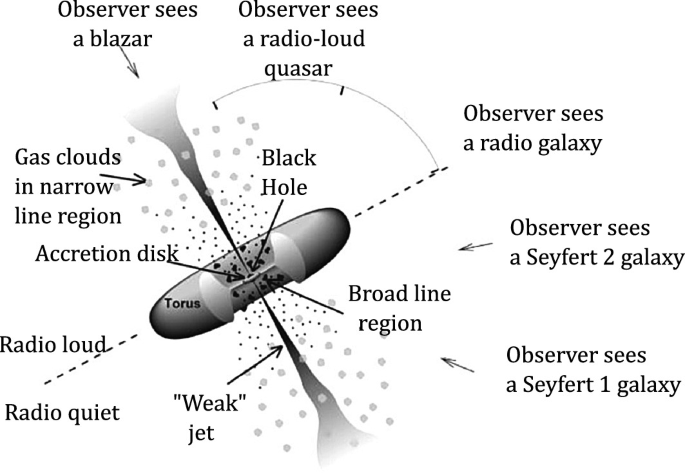
\includegraphics{./figures/nu_he/508900_1_En_8_Fig5_HTML.png}
    \labfig{AGN}
\end{marginfigure}

Active galactic nuclei are extremely bright and compact regions located at the centers of galaxies, powered by supermassive black holes, as shown in \reffig{AGN}. In these regions, surrounding matter forms an accretion disk, where gravitational energy is converted into electromagnetic energy, resulting in the emission of a wide spectrum of radiation (specially when viewed from different directions), from radio waves to gamma rays \sidecite[-8cm]{AGN_picture}. The intense gravitational pull of the black hole compresses the surrounding material, generating high temperatures and pressures. Some AGNs also produce relativistic jets, which are streams of charged particles moving at speeds close to the speed of light. These jets can terminate in hot spots or lobes, providing an environment capable of accelerating cosmic rays to energies nearing 100 EeV \sidecite{Peterson_1997}. 

Gamma-ray bursts, on the other hand, are extremely luminous and transient events characterized by their emission of gamma radiation for brief periods, ranging from milliseconds to several minutes. During their short duration, GRBs emit more energy than any other steady gamma-ray source in the universe \cite{AGN_picture}. Theoretical models describing GRBs, such as the fireball shock model \sidecite{PIRAN1999575}, predict an initial short burst of highly energetic gamma rays followed by a more prolonged afterglow that emits across a broad range of wavelengths, from X-rays to radio frequencies. Long GRBs, which last over 2 seconds, are generally believed to be associated with the core collapse of a massive progenitor star \sidecite{hjorth2011gammarayburstsupernova}. In contrast, shorter GRBs are likely the result of the merger of two neutron stars or a neutron star with a black hole \sidecite{LIGOScientific:2017zic, Janka:1999qu}. In both scenarios, the collapse produces highly relativistic jets that exhibit multiple shock fronts, facilitating the acceleration of cosmic rays to extreme energies.


\section{High Energy Neutrinos}
\label{sec:cosmic_nu}
Cosmic neutrinos are high-energy neutrinos produced through various mechanisms. \textbf{Astrophysical neutrinos} are produced in hadronic interactions within extreme environments like active galactic nuclei and gamma-ray bursts, often in conjunction with cosmic rays. \textbf{Cosmogenic neutrinos} on the other hand, arise from ultra-high-energy protons interacting with the cosmic microwave background, leading to decays that yield neutrinos. Lastly, \textbf{Atmospheric neutrinos} are produced when cosmic rays collide with Earth's atmosphere, initiating air showers that generate mesons like pions and kaons. These mesons decay, leading to the production of neutrinos, along with muons and electromagnetic cascades. 
\todo{figure should change, i can't find citation and i am too lazy to produce one}
\begin{marginfigure}
    \caption{Schematic of progress of a particle cascade when a cosmic ray proton interacts with a nucleus in atmosphere.}
    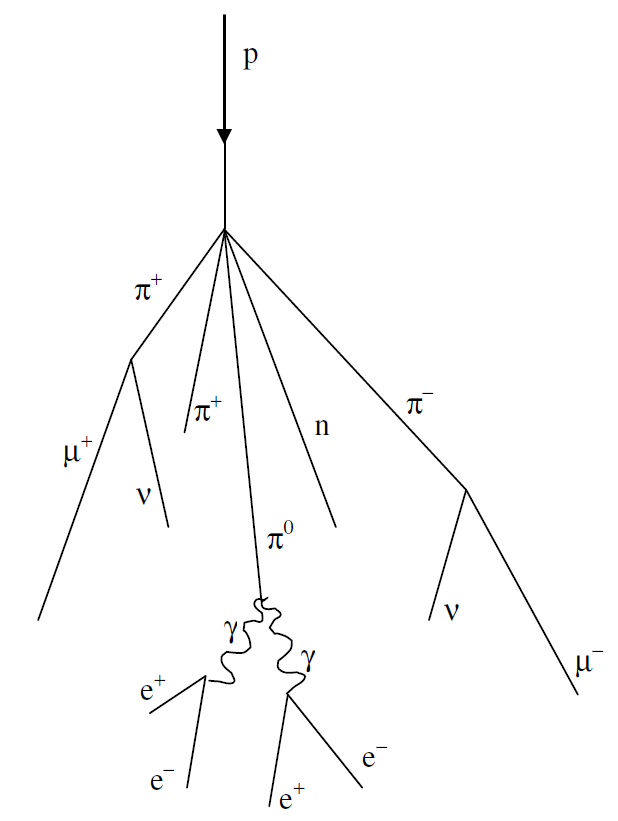
\includegraphics{./figures/nu_he/An-illustration-of-the-Shower-of-Particles-Produced-by-Cosmic-Ray-Collisions-From-Coan.png}
    \labfig{shower}
\end{marginfigure}
Regardless of the location of the source, the basic mechanism of neutirno production of all of the aforementioned neutrinos remains the same, hadronic interactions that producs mesons. The following sections will focus on these neutrino categories, with an emphasis on Astrophysical neutrinos and their production mechanisms, which are most relevant to this thesis.

\subsection{Atmospheric Neutrinos}
\label{sec:atm_nu}
Extensive air showers (EAS) are a cascades of secondary particles initiated when a high-energy primary cosmic ray—such as a proton, neutron, or heavier nucleus—interacts with the Earth's atmosphere. These showers can result from cosmic rays with energies reaching \( E \sim 1 \, \text{PeV} \) and beyond, spreading across areas of approximately 10 km² at ground level \sidecite{Gaisser_2012}. When the cosmic ray collides with atmospheric nuclei, it produces a large number of secondary particles, primarily charged and neutral pions (\(\pi^\pm, \pi^0\)), along with kaons (\(K^\pm, K^0\)) and other mesons.

The dominant fraction of particles in an EAS consists of pions \sidecite{PDG_2024}. Neutral pions (\(\pi^0\)) decay rapidly into photons (\(\pi^0 \rightarrow 2\gamma\)), feeding the electromagnetic component of the shower, which can be observed through detection techniques such as radio emissions, air fluorescence, and Cherenkov light. Charged pions (\(\pi^\pm\)) decay into muons and neutrinos through the processes:
\[
\pi^+ \rightarrow \mu^+ + \nu_\mu, \quad \pi^- \rightarrow \mu^- + \bar{\nu}_\mu,
\]
producing muons and muon-neutrinos. These muons often reach the Earth's surface, where they can be detected by large arrays of particle detectors. If the muons have sufficiently high energy, they can penetrate deep into the ground \sidecite{muon_penetration}, allowing detection by underground observatories like IceCube \sidecite{atm_mu_icecube}. 

The pions and kaons created in the air shower can either decay or interact, resulting in the production of atmospheric muons and neutrinos, which are collectively referred to as the atmospheric muon and neutrino flux.

The energy spectrum of atmospheric neutrinos can be divided into two main categories: conventional and prompt neutrinos. \textbf{The Conventional Atmospheric Neutrinos} are predominantly produced by the decay of charged pions (\(\pi^\pm\)) and kaons (\(K^\pm\)), which are generated in extensive air showers resulting from cosmic-ray interactions with the Earth's atmosphere. The dominant decay channels contributing to the conventional neutrino flux are:\marginnote{\begin{kaobox}
    $K_L^0$ here refers to long-lived neutral kaon which differes from short lived neutral kaon ($K_S^0$) by lifetime and also through decay modes \cite{PDG_2024}. 
\end{kaobox}}
\[
\pi^\pm \rightarrow \mu^\pm + \nu_\mu, \quad K^\pm \rightarrow \mu^\pm + \nu_\mu, \quad K_L^0 \rightarrow \pi^\pm + e^\mp + \nu_e \, (\bar{\nu}_e).
\]
At lower energies (a few GeV), the muons produced in pion and kaon decays usually decay in the atmosphere, leading to an observed flavor ratio of \(\nu_e : \nu_\mu \approx 1:2\). However, at higher energies (above 100 GeV), most muons reach the ground before decaying, significantly reducing the production of electron-neutrinos and causing the flavor ratio to drop below \(1:10\) at TeV energies. This energy-dependent behavior is a key characteristic of the conventional neutrino flux, which dominates in the GeV to TeV range and follows a power law of \(E^{-3.7}\) \cite{PDG_2024}. At energies well above 100 GeV, the contribution of charged pions to the muon-neutrino flux diminishes, and kaon decays become the predominant source of conventional atmospheric neutrinos. Due to the differing decay channels and branching ratios, muon-neutrinos (\(\nu_\mu\)) are produced in much higher numbers compared to electron-neutrinos (\(\nu_e\)), with the flavor ratio \(\nu_\mu : \nu_e\) varying between 20:1 to 30:1 in the TeV to PeV range. 

\marginnote{\begin{kaobox}
    The production of prompt atmospheric tau-neutrinos is highly suppressed and is expected to occur primarily through the decay channel \( D_s^\pm \rightarrow \tau^\pm + \nu_\tau \), followed by the subsequent decay of the tau lepton \( \tau^\pm \rightarrow \mu^\pm + \nu_\mu + \nu_\tau \) \cite{prompt_tau}. The contribution of tau-neutrinos to the overall prompt neutrino flux is approximately 5\% and is generally considered negligible.
\end{kaobox}}

In contrast, \textbf{The Prompt Atmospheric Neutrinos} originate from the rapid decay of charmed mesons (such as \(D^\pm, D^0, D_s^\pm\)), which decay almost immediately after their production without significant interaction. These mesons decay into both muon- and electron-neutrinos via the processes: 
\begin{equation}
    D^\pm \rightarrow \mu^\pm + \nu_\mu , \quad D^0 \rightarrow e^\pm + \nu_e ,
\end{equation}
leading to an expected flavor ratio of \(\nu_\mu : \nu_e \approx 1:1\) for prompt neutrinos. The prompt neutrino flux follows the energy distribution of the primary cosmic ray and is unaffected by atmospheric density. While charmed $D$ mesons contribute to both prompt neutrino and muon fluxes, short-lived vector mesons like, $\eta,\rho,\omega$ may also contribute to prompt fluxes, but only for muons as they usually have dimuonic decay, without any neutrinos \sidecite{ILLANA2011663}.

The atmospheric neutrino energy spectrum is approximately described by two power-law relations:
\[
\frac{dN}{dE} \propto 
\begin{cases}
    E^{-3.7}, & \text{for conventional neutrinos (above 100 GeV)}, \\
    E^{-2.8}, & \text{for prompt neutrinos (below 100 TeV)}.
\end{cases}
\]
The steeper spectrum of conventional neutrinos arises from the fact that charged pions and kaons interact several times before decaying, particularly at higher energies. By contrast, prompt neutrinos, produced directly from the decay of charmed mesons without prior interaction, retain an energy distribution similar to that of the primary cosmic ray. The prompt neutrino flux is also independent of zenith angle, whereas the conventional neutrino flux is most pronounced for neutrinos coming from the horizon, due to the increased probability of pion and kaon decay over longer travel distances through the atmosphere.


The energy spectrum of the conventional atmospheric neutrino flux has been measured up to several hundred GeV by underground experiments like Super-Kamiokande \sidecite{superk_atmflux} and the Fréjus Nucleon-Decay Detector \sidecite{Frejus_ref}, and up to a few hundred TeV by IceCube \sidecite{icecube_nue} and ANTARES \sidecite{antares_atmnu}. However, a prompt atmospheric neutrino flux remains undetected, as the predicted normalization lies below the current detection threshold \sidecite{prompt_tau}. Efforts are underway to combine data samples to improve sensitivity and potentially observe this elusive flux \sidecite{icecube_prompt}. Additionally, IceCube has successfully measured atmospheric muon fluxes up to energies of 1 PeV \sidecite{atm_mu_icecube}.


\subsection{Cosmogenic Neutrinos}
\label{sec:cosmogenic_nu}
As explained in Section~\ref{sec:cosmic_rays}, a cut-off in the energy spectrum of cosmic rays is hypothesized at energies above a few EeV. This cut-off, known as the GZK cutoff, occurs because cosmic-ray protons with energies around 50 EeV are expected to interact with the cosmic microwave background (CMB) photons via the reaction:
\[
p + \gamma_{\text{CMB}} \rightarrow \Delta^+ \rightarrow \begin{cases} p + \pi^0 \\ n + \pi^+ \end{cases}
\]
In this reaction, the resulting $\pi^+$ produced subsequently decays, generating neutrinos that carry a fraction of the original proton energy and thus appear at extremely high energies. These neutrinos are reffered to as \textbf{Cosmogenic Neutrinos} or \textbf{GZK neutrinos}.

The detection of the diffuse extra-galactic gamma-ray background by Fermi LAT, which originates from the decay of the $\pi^0$ produced in the reaction above, further constrains the expected cosmogenic neutrino flux. This constraint imposes an upper limit on the cosmogenic neutrino flux at roughly \( E_\nu^2 \Phi_\nu \lesssim 10^{-8} \, \text{GeV cm}^{-2} \, \text{sr}^{-1} \, \text{s}^{-1} \) for neutrinos near the 1 EeV energy range \sidecite{AHLERS2010106}. However, no neutrinos at such extreme energies have yet been observed by IceCube \sidecite{IceCube:2016uab}.

\subsection{Astrophysical Neutrinos}
\label{sec:astro_nu}
Astrophysical neutrinos are produced alongside cosmic rays, which are accelerated to ultra-high energies in extreme environments. These cosmic rays interact with nearby matter or radiation, resulting in the production of secondary particles that decay into neutrinos. Due to their weak interactions, neutrinos can travel vast distances through space without being absorbed or deflected, making them valuable messengers for tracing the origins of cosmic rays. The production of astrophysical neutrinos can generally be described by two main mechanisms, depending on the type of interaction the cosmic rays undergo.

The \textbf{Hadro-nuclear (pp) Scenario} involves cosmic rays, predominantly protons, colliding with nearby matter, such as dense clouds of interstellar gas composed mainly of hydrogen (neutral or ionized). These proton-proton (pp) interactions are similar to cosmic-ray-induced air showers in the Earth's atmosphere. When a high-energy proton from the cosmic ray flux collides with a thermal proton from the surrounding gas, a cascade of particles is produced, including neutral and charged pions ($\pi^0$, $\pi^\pm$). \marginnote{\begin{kaobox}
    \begin{equation}\label{eq:pi0_decay}
        \pi^0 \rightarrow 2\gamma
    \end{equation}
    \begin{equation}\label{eq:pipm_decay}
        \pi^\pm \rightarrow \mu^\pm + \nu_\mu (\bar{\nu}_\mu)
    \end{equation}
    \begin{equation}\label{eq:muondecay}
        \mu^\pm \rightarrow e^\pm + \barp{\nu_{e}} + \barp{\nu_{\mu}}
    \end{equation}
\end{kaobox}}The neutral pions decay into photons (Equation~\ref{eq:pi0_decay}), while the charged pions decay into muons and neutrinos (Equation~\ref{eq:pipm_decay}), the produced muons subsequently decay, producing more neutrinos and electrons (Equation~\ref{eq:muondecay}). Thus, the hadronuclear scenario results in the production of multiple neutrinos (of both electron and muon flavors) through the decay of charged pions and muons. 

In the \textbf{Photo-hadronic (p$\gamma$) Scenario}, cosmic rays interact with photons, i.e., radiation fields present in the source environment. These interactions, known as p$\gamma$ interactions, lead to the production of pions via, 
\marginnote{\begin{kaobox}
    The p$\gamma$ scenario, explained in Equation~\ref{eq:pgamma} is similar to that described in Section~\ref{sec:cosmogenic_nu} for GZK neutrinos. The difference here is that the photon is much more energetic than that of a CMB photon, hence the threshold energy for the proton to trigger resonance ($\Delta^+$) is much lower.
\end{kaobox}}
\begin{equation}\label{eq:pgamma}
p + \gamma \rightarrow \Delta^+ \rightarrow p(n) + \pi^0(\pi^+),
\end{equation}

Pion production can also happen if the centre of mass energy of $p+\gamma$ is larger than the center of mass energy of the pion. The p$\gamma$ scenario typically occurs in regions with intense radiation fields, such as the jets of AGNs or gamma-ray bursts (GRBs), where high-energy photons are abundant. The produced pions decay similarly to the hadronuclear scenario, generating neutrinos through the same decay chains. 

Each neutrino typically retains about \( \sim \frac{1}{20} \) of the energy of the initial cosmic-ray particle, assuming the primary is a proton and secondary particles decay without additional interactions or significant energy loss \sidecite{fracofenergy}. Consequently, the neutrino energy spectrum is expected to follow a power-law distribution similar to that of the parent cosmic rays , with variations depending on the production mechanism and the nature of the astrophysical source (see Section~\ref{sec:cosmic_rays}). Furthermore, Equations~\ref{eq:pipm_decay} and \ref{eq:muondecay} combined results in a flavor composition of neutrinos at the source given by $\nu_e : \nu_\mu : \nu_\tau = 1 : 2 : 0$. This implies that for every electron neutrino produced, approximately two muon neutrinos are generated, while no tau neutrinos are produced directly at the source. However, due to neutrino oscillations, by the time these neutrinos reach Earth, the flavor composition is expected to evolve into a nearly equal mix of the three flavors ($\nu_e : \nu_\mu : \nu_\tau \approx 1 : 1 : 1$). However, other source combinations are also possible depending on the source and its vicinity, thsi will be discussed in SectionZ\ref{sec:flavor_theory}.

\subsubsection*{Source Candidates}
\label{sec:sources_astro_nu}
One of the main goals of IceCube is to point back to these high energy neutrino sources. Many studies have been made in past, and are on-going to use various event samples to find these high energy source population \sidecite{Naoko_ICRC}. As evident from the discussion above, The simultaneous production of gamma rays and neutrinos implies a tight connection between these messengers within the context of studying cosmic-ray acceleration. A coincidental observation through multi-messenger astronomy and the clear establishment of the connection between the diffuse gamma-ray and neutrino fluxes would be the key ingredients for identifying the sources of cosmic rays. To accomodate such searches, IceCube issues \emph{a realtime alert} of neutrino events that are most promising high energy events \sidecite{realtime}, sending out possible direction and energy of the event to astronomy community, that can further look for events through respective messenger.  

Such an approach gave IceCube its first ever smoking gun signature of a neutrino emitter. the first evidence of an astrophysical neutrino source was the blazar TXS 0506+056, which was spatially coincident with the neutrino alert event IC170922A \sidecite{txspaper}. While the archival neutrino flare further strengthened the case of TXS 0506+056 as a neutrino source, but it was not coincident with enhanced electromagnetic emission \sidecite{txspaper2}. This further poses a problem for the modeling of particle acceleration in blazars \sidecite{Winter:2019hee}. Another search looking for correlations with blazers was conducted using alert events collected over the years, via a catloague serach, which yielded no significant signal, which is compatible with a small fraction (<1\%) of AGNs being neutirno emitter. More recently, strong evidence that the active galaxy NGC 1068 is a neutrino source was found, at the $4.2\sigma$ level \sidecite{ngc1068}. 

Another breakthrough occured recently when IceCube reported observation of neutrino fluxes from the Galactic Plane with a $4.5\sigma$ significance\sidecite{milkyway}. This measurement was revolutionazing as due to location of the IceCube, Because the Galactic center is located in the Southern Sky, diffuse emission is expected to be concentrated in the Southern Sky. IceCube is located at the South Pole, so observations in the southern celestial sky are composed of events downgoing in the detector. Searches in this region are particularly difficult due to the large background of atmospheric muons. Thanks to machine learning techniques, used for careful reconnstruction of the cascade like event, it was possible to make use of a sample, which can improve signal-to-background ratio of these events significantly.

Another proposed source class is \textbf{a Tidal Disruption Event (TDE)}. TDEs are transients that occur when a star passes close to a Supermassive Black Hole (SMBH) and gets disrupted by the tidal force due to the strong gravity. This creates a very bright electromagnetic flare that lasts for months. TDEs have been proposed as high-energy neutrino and ultra-high-energy cosmic ray sources \sidecite{Hayasaki_2021}. A TDE called AT2019dsg was found by the Zwicky Transient Facility (ZTF) in coincidence with the alert \sidecite{Stein_2021}, with a chance probability of 0.5\%. Recently, one more candidate neutrino event has been associated to be coming from a TDE \sidecite{simeon_tde}, making this source class a relevant choice as a contributor to diffuse neutrino fluxes \sidecite{Winter:2022fpf}.

Gamma-ray bursts (GRBs) have long been considered prime candidates for cosmic-ray and associated neutrino production. Neutrino emissions could theoretically occur at various stages of a GRB: during the pre-burst phase of the progenitor star \sidecite{Razzaque:2003uv}, the prompt gamma-ray emission phase \sidecite{Bahcall}, and potentially in the afterglow \sidecite{Waxman:1999ai}. However, early investigations by IceCube showed no significant evidence of high-energy neutrinos linked to gamma-bright GRBs \sidecite{2012}. Further analyses strengthened these findings, indicating that GRBs likely contribute less than about 1\% of the observed diffuse neutrino flux \sidecite{IceCube:2017amx}. This constraint suggests that other sources may play a larger role in the observed astrophysical neutrino fluxes. While individual coincidences with AGNs and starbust galaxy have been established, a conclusive significance to attribute what are the fractional contributions of these source classes to the observed diffusue neutrino fluxes are still remains unknown. Apart from the milkyway observations, all the other mentioned sources hint towards a dominating extragallactic contribution to the observed neutrino fluxes. 

\subsubsection{Diffuse Fluxes}
\label{sec:diffuse_theory}

\textbf{A diffuse astrophysical neutrino flux} results from the collective contributions of numerous faint neutrino sources, each too weak to be individually detected. While multiple classes of sources are likely involved, the specific contributions from each remain unknown. At high-energy sites, as discussed in Section~\ref{sec:astro_nu}, cosmic rays generate neutrinos via \(pp\)- or \(p\gamma\)-interactions in \emph{a beam dump} scenario. This implies a power-law energy spectrum \( dN/dE \sim E^{-\gamma} \) for the neutrino flux, with an approximately isotropic arrival distribution due to the unresolved nature of the sources. 

The neutrino-to-antineutrino ratio is expected to be around \( \nu:\bar{\nu} = 1 \) \sidenote{This assumption may not hold for every individual source. The neutrino-to-antineutrino ratio depends on the abundance of \( \pi^+ \) relative to \( \pi^- \) (or heavier mesons) produced during cosmic ray interactions with the "beam dump." In \( pp \) interactions, charged pions are created in roughly equal amounts, with a slight excess of \( \pi^+ \) due to both cosmic rays and target material being protons. In contrast, \( p\gamma \) interactions produce fewer \( \pi^- \) mesons, primarily through multi-pion production. The limited \( \pi^- \) results in the \( \Delta^+ \) resonance mainly producing \( \nu_\mu \) and \( \nu_e \), while antineutrinos are absent, as shown in Equations \ref{eq:pgamma}, \ref{eq:pipm_decay}, and \ref{eq:muondecay}.} across flavors due to averaging over many sources, though it can vary depending on the charged pion production balance in \( pp \) versus \( p\gamma \) interactions. In the IceCube detector, this ratio is typically indistinguishable, except in cases like the Glashow resonance, where a \( \bar{\nu}_e \) interacts with a detector electron at 6.3 PeV, selectively probing the antineutrino component. See Section~\ref{sec:glashow} for details.

A critical theoretical benchmark for this flux is the Waxman-Bahcall limit, which proposes an upper bound on the neutrino flux if it originates from the same sources responsible for the highest-energy cosmic rays \sidecite{waxman}. According to this bound, if ultra-high-energy cosmic rays are generated in environments that are optically thin to these particles, where most escape before interacting, the corresponding neutrino flux should not exceed:

\begin{equation}\label{waxman_bahcall}
    \Phi(E) \lesssim 3.4\times10^{-8} E^{-2} \, \text{GeV s}^{-1} \, \text{cm}^{-2} \, \text{sr}^{-1} 
\end{equation}
This limit assumes that UHECRs are produced with an \( E^{-2} \) spectrum and that the cosmic-ray production rate aligns roughly with the star formation rate over time. Although some sources that are optically thick to cosmic rays could potentially exceed this bound, they do not naturally account for the origin of UHECRs. Moreover, this limit may get weaker if the observed softer spectrum of the cosmic ray in regions of interest is used instead of the assume harder spectrum \sidecite{PhysRevD.63.023003}.

In the search for astrophysical neutrinos, even a detector like IceCube, burried deep within the antarctic ice sheets, faces a lot of background noise from atmospheric muons and neutrinos created by cosmic-ray air showers, as mentioned in Section~\ref{sec:atm_nu}. IceCube detects about 3,000 muons per second at the trigger level, but typical event selections find only around 10 to 100 astrophysical neutrinos each year, with very few having energies above a few hundred TeV (see e.g., \sidecite{lars_globalfit}). Therefore, the main goal of any event selection is to reduce atmospheric backgrounds enough so that astrophysical neutrinos can be detected. The high rate of muons observed by IceCube is due to the overburden of atmospheric air showers coming straight down the detecto, the so-called \textbf{down-going} region in \reffig{ic_earth}. These poses of course the largest background for astrophysical studies\sidenote{but are a great source to study cosmic ray air showers}. Ideally, one could look for events that only come from the so-called \textbf{up-going} region, as shown in the \reffig{ic_earth}, where the produced muons and neutrinos in air-showers shall be reduced significantly, as these neutrinos would have to travel through earth to reach the detector, which most of them don't survive. This solution comes at a cost of loosing half of the sky. An alternative solution is to use events that start within the instrumentation volume, but uses outer layer of the detctor to \emph{veto} these muons and neutrinos from the air showers. Such an event sample is used for the analysis presneted in this thesis and will be dicussed in great detail in \refch{nu_samples}.

\begin{figure}[h!]
    \caption{The measured energy spectra of atmospheric and cosmic diffuse neutrino fluxes have been obtained. Experimental limits at the highest energies are compared with model predictions for cosmogenic neutrinos. All fluxes are normalized to a single flavor ($\nu + \bar{\nu}$), assuming a ratio of $\nu : \bar{\nu} = 1$, and for cosmic neutrinos, a ratio of $\nu_e : \nu_\mu : \nu_\tau = 1 : 1 : 1$ at Earth. Each measurement is referenced in \cite{PDG_2024}}
    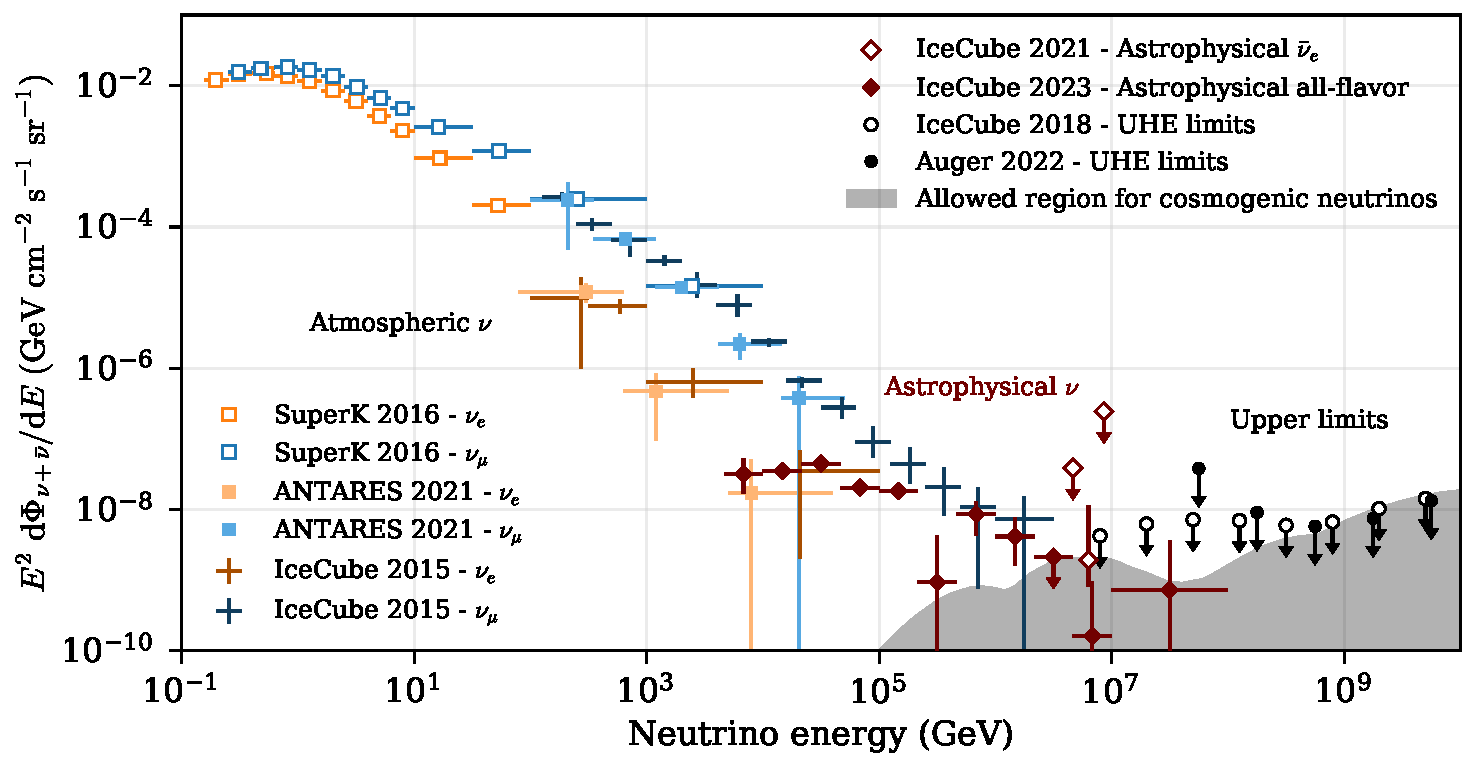
\includegraphics{./figures/nu_he/neutrino_spectrum_wide_231010.pdf}
    \labfig{nu_fluxes}
\end{figure}
\todo{add the earth schematic to show up and down going regions here}

The aforementioned sample, that uses outer layer of the detector as veto was used to find an evidence for astrophysical neutrinos was first observed by IceCube in 2013 \sidecite{Evidence_paper}. While subsequent analyses reinforced this discovery \sidecite{HESE4,HESE6}, different studies using various event samples revealed power-law indices spanning from \( E^{-2} \) to \( E^{-3} \), suggesting potential substructures within the flux \sidecite{diffusenumu,cscd_6yr,lars_globalfit,HESE7_sample}. Although initial data hinted at these features, two recent independent IceCube studies confirmed a spectral break in the neutrino spectrum: hardening below 30 TeV and softening at higher energies, with a broken power law preferred over a single power law with more than \( 4\sigma \) significance \sidecite{globalfit_icrc,MESE_ICRC}. This spectral break offers key insights into the underlying astrophysical neutrino production mechanisms. 

%SuperK 2016 [243]; ANTARES 2021 [244]; IceCube 2015 νe [245]; IceCube 2015 νμ [246]; IceCube 2021 astrophysical ν ̄e (ν + ν flux derived from a single candidate event for the Glashow resonance) [247]; IceCube 2023 astrophysical all flavor [39]. The limits at the highest energies are taken from [248] (IceCube) and [249] (Auger).

\reffig{nu_fluxes} shows the most updated measurements for both atmospheric and astrphysical fluxes of neutrinos, along with limits at higher energies for cosmogenic neutrinos. 

\subsubsection{Flavour Composition}
\label{sec:flavor_theory}


As outlined in Section~\ref{sec:astro_nu}, neutrinos are produced via the decays of charged pions and muons, leading to the generation of only $\nu_e$ and $\nu_\mu$ in various interaction scenarios.

\marginnote{\begin{kaobox}
Flavor composition, or alternatively called the flavor ratio, is described as a set of three numbers, $(f_e : f_\mu : f_\tau)$, often normalized so that $f_e + f_\mu + f_\tau = 1$, representing the fraction of each neutrino flavor in the astrophysical flux.
\end{kaobox}}

The flavor composition of neutrinos can significantly vary depending on the environments of high-energy sources. For instance, produced pions and muons may interact before decaying, thereby altering the expected neutrino ratios. This leads to several \textbf{source scenarios}, each resulting in different overall flavor compositions.

The scenario discussed in Section~\ref{sec:astro_nu} describes the \textbf{pion production scenario}, where the source environments are assumed to be sparse enough that the produced muons and pions do not interact with matter before decaying. In this case, the expected flavor composition at the source would be $\nu_e:\nu_{\mu}:\nu_{\tau} = 1:2:0$.


In high-radiation or magnetic field environments, charged pions and muons from $pp$ and $p\gamma$ interactions can undergo significant synchrotron energy losses, around $(m_p/m_{\pi,\mu})^3 \sim 10^3$ times greater than for protons. Given their $\tau_\mu/\tau_{\pi^\pm} \sim 10^2$ times longer lifetimes \sidecite{PDG_2024}, muons are more likely to interact before decaying, rendering these sources opaque to muons and thus eliminating their contribution to the neutrino flux. In this \textbf{muon-damped scenario}, the source flavor composition shifts to $\nu_e : \nu_\mu : \nu_\tau = 0 : 1 : 0$. Since muon interaction probability increases with energy, a realistic model would show an energy-dependent shift in flavor composition from $1 : 2 : 0$ to $0 : 1 : 0$ over 1-2 decades in energy, expected around $\sim 100$ TeV for GRBs \sidecite{cite166}.

Additionally, in sources with dominant $p\gamma$ interactions and extremely strong magnetic fields, the \textbf{neutron-beam scenario} leads to a flavor composition of $\nu_e : \nu_\mu : \nu_\tau = 1 : 0 : 0$ \sidecite{cite167}. Here, highly energetic neutrons are produced, either through processes like those in Equation~\ref{eq:pgamma} or by photodisintegration of heavy cosmic-ray nuclei. For neutrons to decay via $n \rightarrow p + e^- + \bar{\nu}_e$, the source environment must be optically thin, as the resulting $\bar{\nu}_e$ are generally lower in energy compared to neutrinos from charged pion or muon decay. Strong magnetic fields are also needed to cool charged pions and muons through synchrotron losses, preventing their decays from contributing to the high-energy neutrino spectrum.

For sources with dominant $pp$ interactions at very high energies, heavier mesons such as charmed mesons can form. This \textbf{charm-production scenario} has a flavor composition of $\nu_e : \nu_\mu : \nu_\tau = 1 : 1 : 0$ \sidecite{prompt_tau}, similar to the production of prompt atmospheric neutrinos (see Section~\ref{sec:atm_nu}). Here, charmed $D$-meson decay produces equal amounts of $\nu_e$ and $\nu_\mu$, with tau neutrinos contributing about 5\%, which can be neglected. While heavier mesons could form, bottom mesons are produced at roughly 10 times lower rates than charmed mesons \sidecite{cite59}. This composition, $\nu_e : \nu_\mu : \nu_\tau = 1 : 1 : 0$, can also arise from energy-dependent secondary acceleration of muons and pions at the source \sidecite{cite168}.

In general, realistic sources likely exhibit varying flavor compositions that depend on energy and the source environment \sidecite{cite169}. These scenarios fit within a broader model that parameterizes flavor composition by the size and magnetic field of the acceleration region in the Hillas phase space \sidecite{cite170}, incorporating synchrotron cooling and high-energy processes to suggest a range of energy-dependent transitions among individual cases.

Due to neutrino oscillations, the flavor composition undergoes changes as neutrinos travel from source to observer. Astrophysical neutrinos are likely produced incoherently in the scenarios described above, possessing varying energies at different locations near the source and traversing cosmic distances before detection on Earth.

Recall the transition probability for neutrino oscillations, where a neutrino from flavor eigenstate $\alpha$ can be measured in flavor eigenstate $\beta$ as expressed in Equation~\ref{eq:main_probability}:

\[
P(\nu_\alpha \to \nu_\beta) = |U_{\alpha j}| |U_{\beta j}| + 2 \text{Re}(U_{\alpha j} U_{\beta j} U_{\alpha k} U_{\beta k} e^{i \Delta m^2 L / 2E}),
\]

where separating diagonal and off-diagonal terms leads to:

\[
\langle P(\nu_\alpha \to \nu_\beta) \rangle = X |U_{\alpha j}|^2 |U_{\beta j}|^2.
\]

This result is independent of $\Delta m^2$, $E$, and $L$, meaning that the expected astrophysical neutrino flavor composition at Earth is fully determined by the emitted composition at the source and the mixing parameters $\theta_{12}, \theta_{23}, \theta_{13}$, and $\delta_{CP}$.
\begin{figure}[h]
    \caption{The measured flavor composition of IceCube's high-energy starting events (HESE) is shown. The contours represent the $1\sigma$ and $2\sigma$ confidence intervals. Shaded regions indicate previously published results \cite{lars_globalfit,gary_paper}, which lacked direct sensitivity to the tau neutrino component. Expected flavor compositions for various astrophysical neutrino production mechanisms discussed in text marked on the figure. Figure from \cite{Juliana_paper}}
    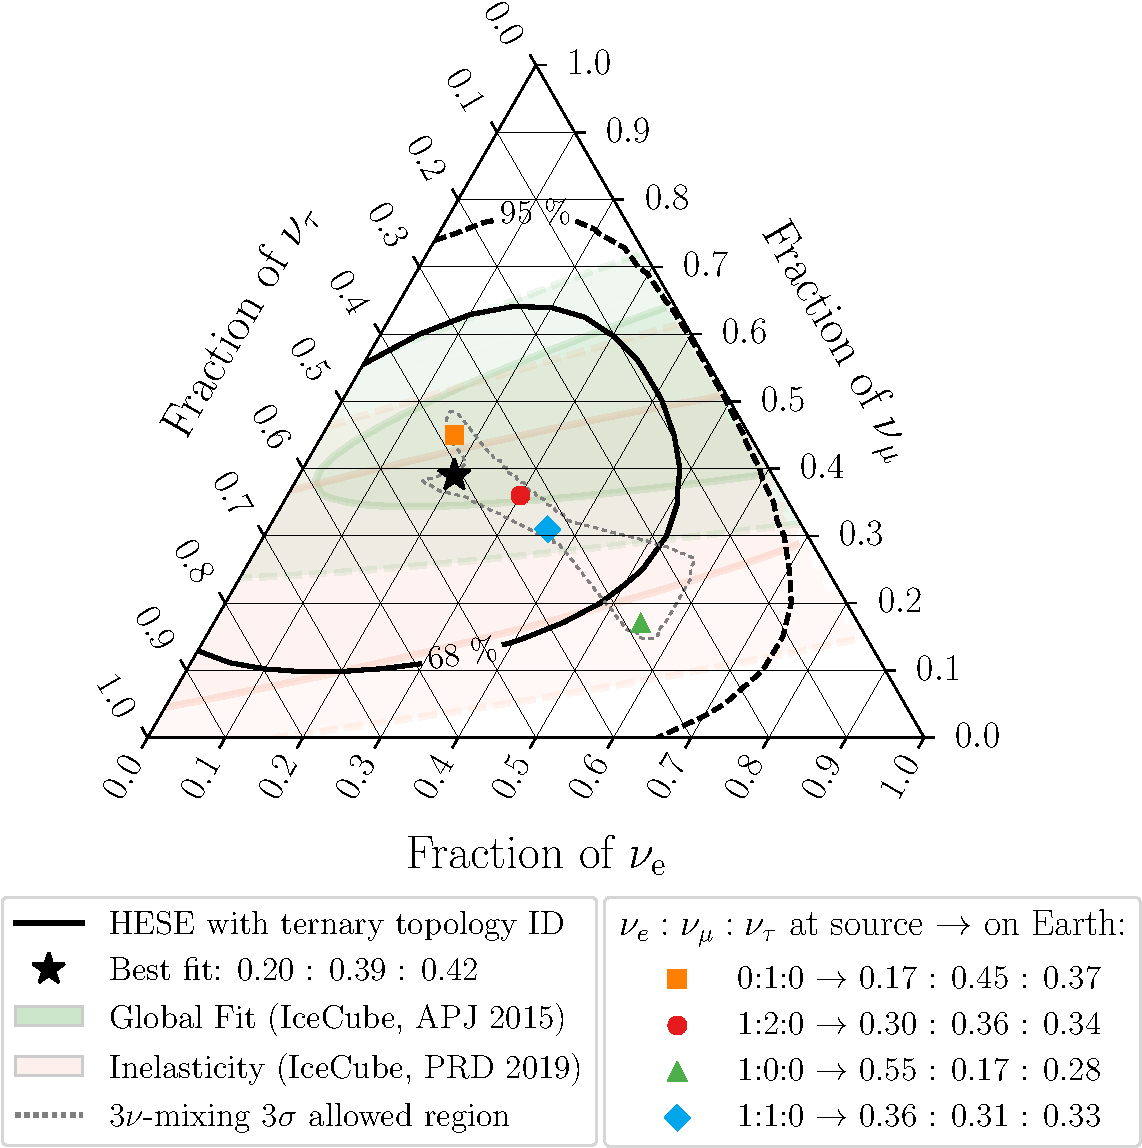
\includegraphics{./figures/nu_he/flavor_scan_7yr_steps21_inel_gf_source_shaded_serif_paper.pdf}
    \labfig{flav_triangle}
\end{figure}
Utilizing the current best-fit measurements detailed in Table~\ref{mixing_parameters}, we can derive the measured flavor ratios for the various scenarios:

\begin{kaobox}
\centering
\textbf{Pion-production scenario:} $1 : 2 : 0 \rightarrow 0.31 : 0.35 : 0.34$\\ 
\textbf{Muon-damped scenario:} $0 : 1 : 0 \rightarrow 0.19 : 0.43 : 0.38$\\ 
\textbf{Neutron-beam scenario:} $1 : 0 : 0 \rightarrow 0.55 : 0.19 : 0.26 $\\
\textbf{Charm-production scenario:} $1 : 1 : 0 \rightarrow 0.37 : 0.31 : 0.32$\\
\end{kaobox}

Despite the vast range of conceivable neutrino flavor compositions associated with cosmic rays, the detectable altered compositions on Earth are confined to a narrow phase space, as shown by the dotted grey lines around various colorful points in \reffig{flav_triangle}. Moreover, this region encompasses the uncertainties in the mixing parameters at the $3\sigma$ confidence level. This result has two notable implications: first, the limited phase space of detectable flavor compositions at Earth suggests that high-precision measurements are crucial for excluding specific source models. Second, any production scenario predicts that the detectable astrophysical tau-neutrino fraction at Earth will be significantly greater than zero.

This makes flavor measurement of astrophysical neutrinos an intriguing probe for examining source contributions to the diffuse neutrino spectrum. Several studies within IceCube have attempted to measure this flavor ratio, as shown in \reffig{flav_triangle}. As emphasized earlier, and visible in the figure, the main factor in measuring flavor composition is identifying tau neutrino events, since regardless of the favored scenario, a non-zero tau fraction is expected. The flavor triangle in \reffig{flav_triangle} illustrates a measurement using three distinct IceCube samples \sidecite{lars_globalfit,gary_paper,Juliana_paper}, where only the most recent measurement, which used the all-flavor starting event sample \cite{Juliana_paper}, achieved the first-ever non-zero $\nu_\tau$ fraction by identifying two tau neutrino candidates in IceCube. A subsequent study used a \emph{convolutional neural network (CNN)} approach to search for $\nu_\tau$ events and found 7 $\nu_\tau$ candidates in IceCube data \sidecite{CNN_tau}, ruling out the absence of an astrophysical $\nu_\tau$ flux at the $5\sigma$ level. The measurement of neutrino flavors in astrophysical sources, aimed at in this thesis, seeks to further refine these observations and provide crucial insights into the flavor composition of the diffuse neutrino spectrum.

